\subsection{Vocoders} \label{sec:vocoders}

\Ac{DL} vocoders are neural network models that have the ability to generate artificial audio~\cite{mehrish_review_2023}. These models employ deep learning networks to learn the mapping between the input and waveform data directly. There is no reliance on any predefined model or feature extraction method. This approach has the ability to capture complex nonlinear relationships between input and output representations that are difficult to be modeled analytically.

There are different types of \ac{DL} vocoders, depending on the input and output representations they use. Some use Mel-spectrum features as conditioning inputs, while others do not require explicit features and directly generate raw waveform samples.

These models can achieve high quality and naturalness of audio synthesis, but they also face some challenges that limit their applicability. One challenge is the high computational cost of generating raw waveform samples at high sampling rates, which requires many computation and memory resources. This limits the scalability and efficiency of these models for real-time applications. Another challenge is the need for high-quality audio data with consistent annotations. This makes training these models with sufficient data diversity and coverage difficult. A third challenge is the generalization problem of these models, which tend to overfit the training data.

\subsubsection{WaveNet} \label{sec:wavenet}

\textit{WaveNet} is a generative neural network developed by DeepMind in 2016. It uses a unique architecture based on dilated causal convolutions to generate raw audio waveforms \cite{oord_wavenet_2016}. It implements the PixelCNN (see Section \ref{sec:pixelcnn}) model for sound and follows an \ac{AR} architecture (see Section \ref{sec:darn}) with the predictive distribution for each audio sample being conditioned on a window of previous ones.

WaveNet's structure allows it to process input sequences in parallel, enabling it to model long context dependencies, even with thousands of timesteps. It uses a series of dilated convolutional layers, where the dilation rate is increased with each layer, which effectively increases the receptive field of the network without increasing the number of parameters.

A dilated convolution happens when the filter is applied over an area larger than its length by skipping input values with a specific step \cite{oord_wavenet_2016}. This architecture can be seen in Figure \ref{fig:dilated-convolution}.

\begin{figure}[ht]
    \centering
    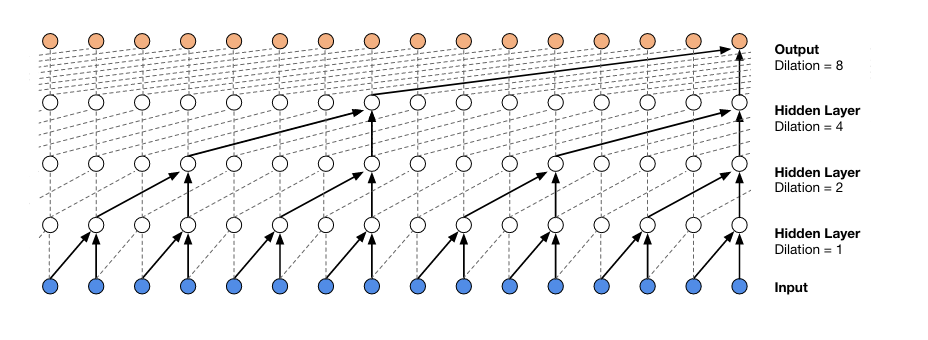
\includegraphics[width=\textwidth]{figures/2-sota/dilated-convolution.png}
    \caption[WaveNet]{\textbf{WaveNet} --- This illustration was taken from \cite{oord_wavenet_2016}. It shows the idea behind WaveNet, applying dilated convolutions to \ac{AR} models.}
    \label{fig:dilated-convolution}
\end{figure}

This structure enables WaveNet to capture long-range dependencies in the input sequence, which is crucial for generating high-quality audio. If an \ac{RNN} (see Section \ref{sec:rnn}) sees only one input sample at each time step, WaveNet has direct access to multiple input samples \cite{huzaifah_deep_2021}. For example, in speech generation, WaveNet can use its sizeable receptive field to model the relationship between a word spoken early in a sentence and its pronunciation later in the sentence.

WaveNet uses a softmax activation function at each output node to produce a probability distribution over the possible values at each time step. During training, the network is fed sequences of input data and their corresponding ground truth values. The model's parameters are adjusted so that its outputs match the ground truth as closely as possible.

WaveNet can use its trained parameters to generate new sequences by sampling from its output probability distribution during generation. This allows it to generate diverse and high-quality outputs, such as realistic human speech or written text, by combining its learned representations of the underlying data distribution with a small amount of randomness.

The input of WaveNet is usually a Mel-Spectrogram (or other representations), and the output is the sound signal.

WaveNet can be conditioned on, for instance, text for \ac{TTS} settings by feeding extra information about the text itself (\textit{e.g.} embeddings). If a model is not conditioned on text, it generates random sounds without any global structure behind it.

The results were astonishing. ``A single WaveNet can capture the characteristics of many different speakers with equal fidelity, and can switch between them by conditioning on the speaker identity. When trained to model music, we find that it generates novel and often highly realistic musical fragments.'' \cite{oord_wavenet_2016}.

Even though this model is good at learning the characteristics of sounds over brief periods, it struggles with global latent structure. They are also very slow for training and inferring \cite{tahiroglu_-terity_2020}.

%%%%%%%%%%%%%%%%%%%%%%%%%%%%%%%%%

\subsubsection{WaveNet Variants} \label{sec:wavenet-variants}

The WaveNet model has emerged as a powerful tool for generating high-quality audio waveforms, particularly for speech and music applications. However, its architecture, which employs dilated convolutions and deep residual networks, can be computationally intensive and challenging to train. To address these limitations, several WaveNet variants have been proposed in recent years that aim to reduce the complexity of the model while maintaining its effectiveness.

One such variant is \textbf{WaveRNN} \cite{kalchbrenner_efficient_2018}, which employs a single \ac{RNN} (see Section \ref{sec:rnn}) to approximate the dilated convolutions in WaveNet. This approach significantly speeds up training time while maintaining the quality of the generated audio. Another variant, FloWaveNet \cite{kim_flowavenet_2018}, employs a flow-based generative model (Section \ref{sec:flow-model}) that allows for efficient training with only one training stage while producing high-quality audio. Additionally, Fast WaveNet  \cite{paine_fast_2016} employs a caching mechanism to reduce the computational cost of the model while maintaining an \ac{AR} structure.

These WaveNet variants are unique in their architectures and training procedures but share the goal of making audio generation more efficient and accessible. While these models are primarily focused on speech and music generation, they can be adapted to other types of audio data. Ongoing research in this area may explore further optimization of these models, integration with other models, and application to new domains.

\subsubsection{MelGAN} \label{sec:melgan}

According to Kumar et al. in 2019, in their \textit{MelGAN} paper~\cite{kumar_melgan_2019}, audio generation with \acp{GAN} is possible although a challenging task (see Section \ref{sec:gan}). Previous studies in this field have encountered difficulties generating coherent raw audio waveforms using \acp{GAN}. Nonetheless, Kumar et al. demonstrate in their \textit{MelGAN} paper that introducing certain architectural changes makes it feasible to train \acp{GAN} to generate high-quality and coherent audio waveforms reliably.

The generator of MelGAN is a fully convolutional feed-forward network that takes a Mel-Spectrogram as input and generates a raw waveform as output. This approach allows for efficient and parallelized processing of audio data.

The decoder takes the waveform and decides whether it is a realistic sound. The decoder is not a single neural network but a multi-scale architecture with three discriminators (D1, D2, D3). These discriminators have identical network structures but operate on different audio scales. D1 operates on the scale of raw audio, while D2 and D3 operate on raw audio downsampled by a factor of 2 and 4, respectively. The use of multiple discriminators at different scales is motivated by the fact that audio has structure at different levels.

MelGAN proved itself way faster than other architectures such as WaveNet (see Section \ref{sec:wavenet}) with comparable results (for inference, roughly thirty-six thousand times faster than WaveNet), given its reduced number of parameters.


%%%%%%%%%%%%%%%%%%%%%%%%%%%%%%%%%

\subsubsection{GANSynth} \label{sec:gansynth}

\textit{GanSynth}, presented in 2019, \cite{engel_gansynth_2019} is a \ac{GAN} (see Section \ref{sec:gan}) that uses log-magnitude spectrograms and phases to generate coherent waveforms. Compared to directly generating waveforms with stridden convolutions, the use of spectrograms and phases has been shown to produce better results.

The study focuses on the NSynth \cite{engel_neural_2017} dataset, a collection of 300 000 musical notes from 1 000 different instruments.

The model first samples a random vector $z$ from a spherical Gaussian distribution. This vector is passed through a stack of transposed convolutions, which upsample and generate output data $x = G(z)$. This generated data is then fed into a discriminator network, which uses downsampling convolutions to estimate a divergence measure between the real and generated distributions.

The architecture of the discriminator network mirrors that of the generator, which allows for a more efficient training process. Optimizing the divergence measure allows the generator to produce spectrograms and phases that resemble actual musical notes more closely.

The study results demonstrate that \acp{GAN} outperform WaveNet (see Section \ref{sec:wavenet}) baselines on automated and human evaluation metrics and can efficiently generate several audio orders of magnitude faster than their \ac{AR} counterparts.

%%%%%%%%%%%%%%%%%%%%%%%%%%%%%%%%%

\subsubsection{HiFi-GAN}

Proposed in 2020, \textit{HiFi-GAN} \cite{kong_hifi-gan_2020} is a \ac{GAN} (see Section \ref{sec:gan}) model that combines efficiency and high-fidelity speech synthesis. HiFi-GAN achieves this by leveraging the periodic patterns inherent in speech audio, demonstrating that modeling these patterns is crucial for enhancing sample quality. The model includes a generator and two discriminators, trained adversarially, and two additional losses for improving training stability and model performance.

The generator is a fully \ac{CNN} (see Section~\ref{sec:CNN}) that takes Mel-Spectrograms as input and upsamples them through transposed convolutions, matching the temporal resolution of raw waveforms. The discriminators are the \ac{MSD} and a \ac{MPD}. \Ac{MSD} evaluates the audio sequence on different scales using a mixture of three convolutional sub-discriminators with different average pools. At the same time, \ac{MPD} consists of small sub-discriminators that capture different implicit structures of input audio by looking at different parts, accepting only equally spaced samples of input audio with different periods. 

HiFi-GAN's performance is evaluated using a subjective human evaluation (\ac{MOS}) on a single speaker dataset, which shows that the proposed method exhibits similarity to human quality. The model achieves a higher \ac{MOS} score than WaveNet (see Section \ref{sec:wavenet}).

Importantly, HiFi-GAN achieves this high-quality synthesis efficiently. Specifically, the model generates 22.05 kHz high-fidelity audio 167.9 times faster than real-time on a single V100 \ac{GPU}, demonstrating superior computational efficiency compared to AR and flow-based models. Moreover, a small-footprint version of HiFi-GAN generates samples 13.4 times faster than real-time on \ac{CPU} with comparable quality to an \ac{AR} counterpart.
